\chapter{Implementation Details}
This chapter describes how the system was built. Section~5.1 states the development environment. Section~5.2 describes the datasets and their sources. Section~5.3 describes the model implementation and how the client and service share it. Section~5.4 records the evaluation metrics and the steps taken for reproducibility. Section~5.5 presents the delivered application.

\section{Development Environment}
The project is a single repository with two overlapping workspaces. A pnpm workspace holds the TypeScript client and the shared client-side engines, and a uv workspace holds the Python packages, the intelligence service, and the offline research code. The two coexist so that the research code can import the same Python engines the service runs, which keeps the evaluated code and the shipped code identical. Table~\ref{tab:tools} lists the environment.

\begin{table}[htbp]
\centering
\footnotesize
\caption{Development environment: tools and libraries.}
\label{tab:tools}
\begin{tabular}{p{4.0cm} p{8.4cm}}
\toprule
\textbf{Concern} & \textbf{Technology} \\
\midrule
Client language and build & TypeScript, Vite, pnpm workspace \\
Client UI & React~19 \\
Local-first storage & Dexie over IndexedDB \\
Intelligence service & Python~3.12, FastAPI, Uvicorn \\
Scientific stack & NumPy, SciPy \\
Service authentication & PyJWT, verifying Supabase-issued tokens \\
Containerisation & Docker via Colima \\
Python workspace & uv \\
JavaScript testing & Vitest, fast-check (property tests), Playwright (end-to-end) \\
Python testing and linting & pytest, ruff \\
Backend and hosting & Supabase (auth, database, storage), Vercel \\
\bottomrule
\end{tabular}
\end{table}

\section{Datasets and Their Sources}
Because a single learner's real log cannot supply a known ground truth, the comparison in Chapter~6 is run on synthetic data whose properties are planted and therefore known. Table~\ref{tab:datasets} lists the datasets and the role each plays.

The synthetic generator produces study histories in which the learner's true pace, the timing and size of any regime shift, and the completion behaviour are set explicitly. So that the synthetic regime resembles real behaviour rather than an arbitrary one, its parameters were calibrated against the Open University Learning Analytics Dataset (OULAD), a large public dataset of learner activity. The OULAD is used only to calibrate the generator's realism; it is not used as a direct benchmark. A revised generator regime models the booking interaction pattern introduced by the redesign of Section~4.4, and the selected models were re-checked against it. Real single-learner logs are reserved for the longitudinal validation planned in Phase~II and are not used in Phase~I.

\begin{table}[htbp]
\centering
\footnotesize
\caption{Datasets used in Phase~I and their sources.}
\label{tab:datasets}
\begin{tabular}{p{3.6cm} p{3.8cm} p{5.0cm}}
\toprule
\textbf{Dataset} & \textbf{Source} & \textbf{Role} \\
\midrule
Synthetic study histories & Generated in-repository & Primary ground truth for the component comparison; plants pace, shifts, and learner archetypes \\
OULAD & Public (Open University) & Calibrates the synthetic generator's realism regime; not a direct benchmark \\
Revised (decoupled) regime & Generated in-repository & Re-validates the selected models under the booking interaction model \\
Real single-learner log & The candidate's own sessions & Phase-II longitudinal validation; not used in Phase~I \\
\bottomrule
\end{tabular}
\end{table}

\section{Model Implementation}
The algorithms are implemented once in behaviour and twice in code. The client-side engines are written in TypeScript, and a Python mirror of each engine is exposed through the intelligence service. The two implementations are kept aligned by a golden-fixture parity harness: the TypeScript engines emit reference inputs and outputs, and a Python test replays each input and asserts numeric equality to a tight tolerance. The shared numeric constants, such as the Bayesian prior, the CUSUM slack and threshold factors, and the Gaussian-process length scale, are held identical on both sides.

The split between client and service follows the architecture of Figure~\ref{fig:arch-revised}. Computation that fits a statistical model to accumulated history runs on the service: Bayesian and enriched-shrinkage pace calibration and CUSUM change detection, reached over HTTP at a calibration endpoint that verifies a signed token before running. Computation that derives a view from the local event log runs in the browser: the Gaussian-process projection, the burn-up and streak summaries, and the capacity-based booking engine. The offline research harness imports the production Python engines as candidates rather than re-implementing them, so a result measured offline is a result about the shipped code. Listing~\ref{lst:cusum} shows the shipped change detector, which realises Equation~\eqref{eq:cusum}, and Table~\ref{tab:packages} lists the main packages.

\noindent\begin{minipage}{\linewidth}
\begin{lstlisting}[language=Python, caption={The shipped one-sided CUSUM detector, realising Equation~\eqref{eq:cusum}.}, label={lst:cusum}]
def run_cusum(series, mu0, k, h):
    """Return the index of the first alarm, or None if no shift is detected."""
    s = 0.0
    for t, x in enumerate(series):
        s = max(0.0, s + (x - mu0) - k)   # accumulate deviation, floored at zero
        if s > h:                          # threshold crossed -> shift detected
            return t
    return None
\end{lstlisting}
\end{minipage}

\begin{table}[H]
\centering
\footnotesize
\caption{Main packages and their roles.}
\label{tab:packages}
\begin{tabular}{p{4.8cm} p{7.6cm}}
\toprule
\textbf{Package / module} & \textbf{Role} \\
\midrule
\texttt{packages/progress} (TS) & Client engine: Gaussian-process projection, burn-up, streak, calibration mirror \\
\texttt{packages/roadmap-engine} (TS) & Client booking and roadmap generation \\
\texttt{packages/py-progress} (Py) & Python mirror: Bayesian and enriched-shrinkage calibration, CUSUM, Gaussian process \\
\texttt{packages/py-roadmap-engine} (Py) & Python mirror of the roadmap engine \\
\texttt{services/intelligence} (Py) & FastAPI service exposing calibration over HTTP, token-verified \\
\texttt{research/comparison} (Py) & Offline harness importing the production engines as candidates \\
\bottomrule
\end{tabular}
\end{table}

\section{Evaluation Metrics and Reproducibility}
The metrics used to score each component are defined in Table~\ref{tab:metrics} of Chapter~4: recovery error for calibration, detection latency and false-alarm rate for change detection, interval coverage and point error for projection, and deadline drift and capacity violations for scheduling. This section records how they are computed and how the results are made reproducible.

Every reported comparison is accompanied by a bootstrap confidence interval on the difference between a candidate and the incumbent, estimated by resampling learners with replacement. Across the family of comparisons a Holm or Benjamini--Hochberg correction is applied, so that a claimed win survives multiple-comparison scrutiny rather than arising from testing many candidates. A result is reported only when it passes a set of credibility checks that guard against degenerate or unstable cells. The pipeline is driven by fixed random seeds and a small set of make targets, so that the dataset, the comparison, and the figures regenerate deterministically, and each generated figure and table carries a provenance stamp recording the run that produced it.

\section{The Phase-1 Application}
The methodology is realised in a working, local-first web application for a single self-directed learner. A new learner is taken through a short onboarding flow that collects a deadline, a weekly study capacity, and a set of materials, and produces an initial plan of bookings (Figure~\ref{fig:app-onboarding}). During study the learner runs a session from a booking, choosing the material at the start and working under a timer with optional Pomodoro intervals (Figure~\ref{fig:app-session}). The Home dashboard summarises the current state: the up-next booking, the study streak, the calibrated pace, and the projected finish date (Figure~\ref{fig:app-home}). The Week view reports the week's verdict alongside a daily-minutes chart and the burn-up projection (Figure~\ref{fig:app-week}). When the projection diverges from the deadline, the Replan screen offers the learner three levers to adjust the plan (Figure~\ref{fig:app-replan}). The Roadmap calendar shows the plan as a month grid of bookings (Figure~\ref{fig:app-roadmap}), and the Roadmaps dashboard tracks the active plan and past plans over their lifecycle (Figure~\ref{fig:app-roadmaps}).

The screenshots below are captured from the running application.

\begin{figure}[htbp]
\centering
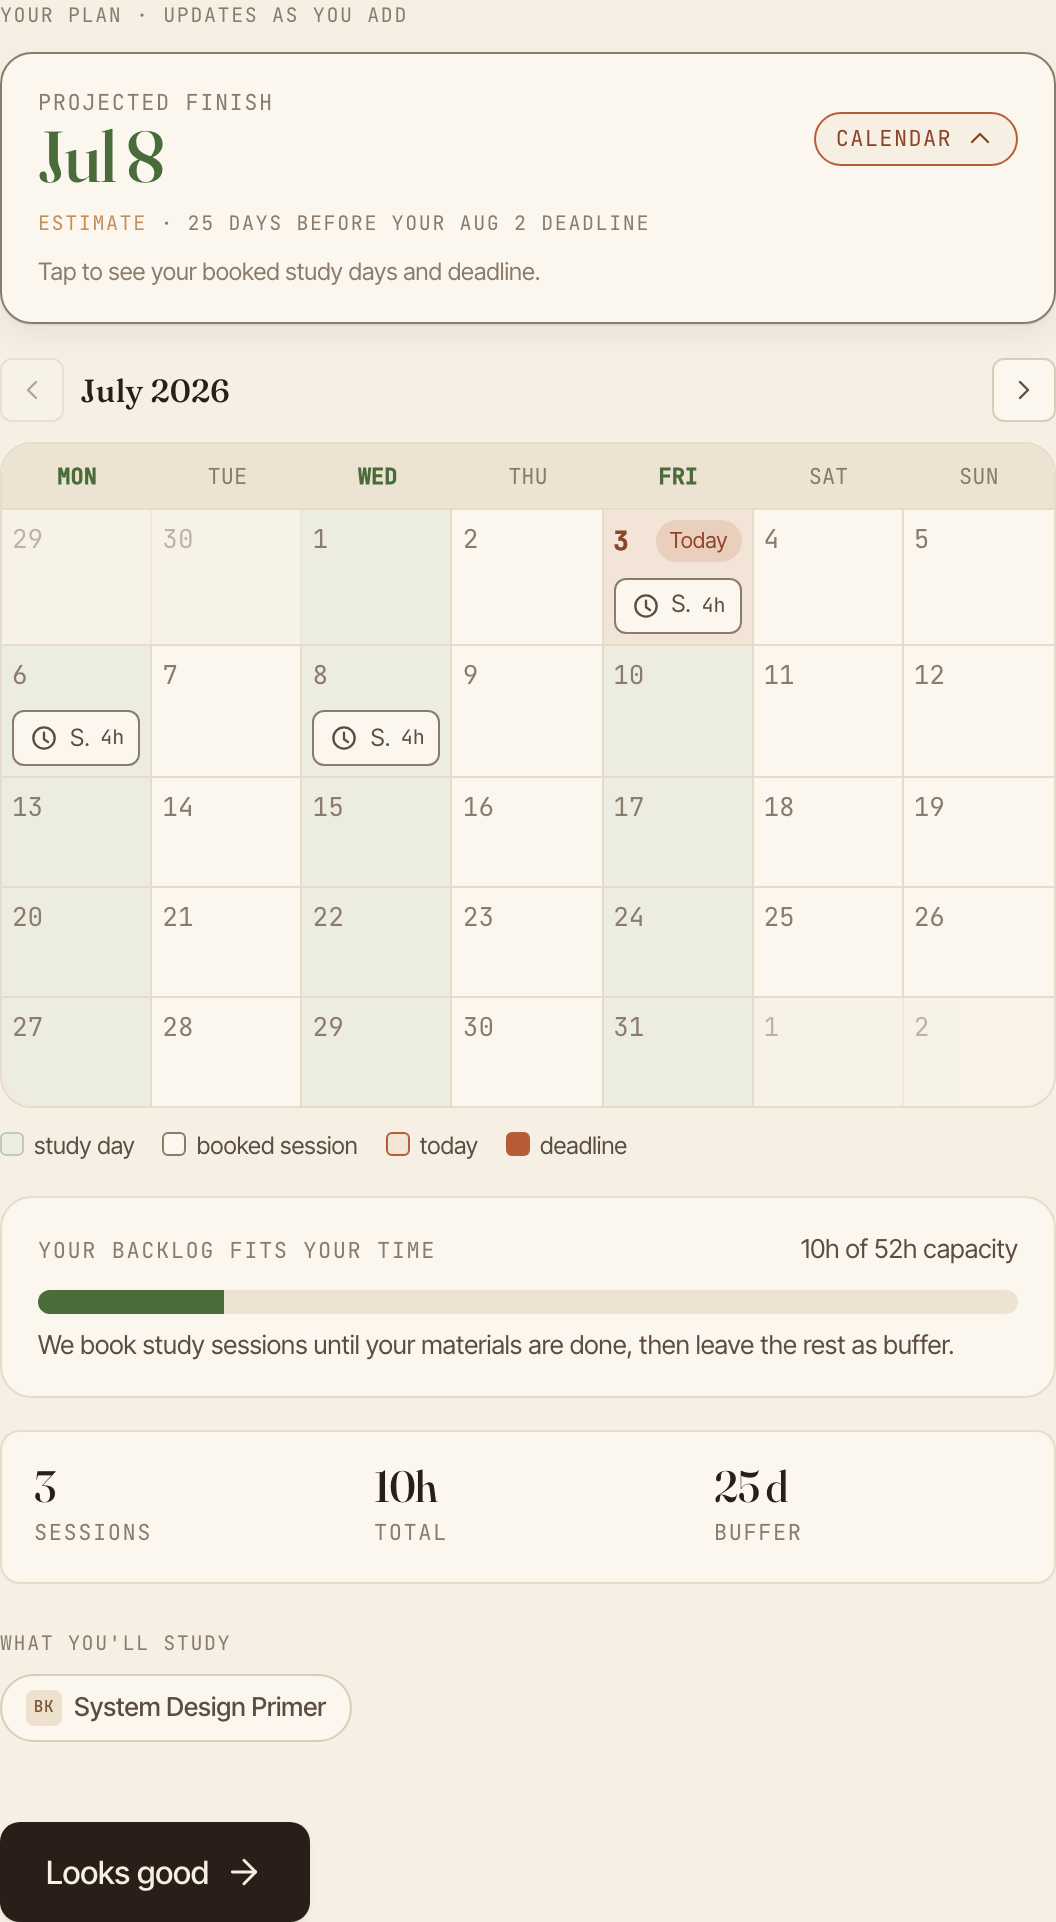
\includegraphics[width=0.85\linewidth, height=0.42\textheight, keepaspectratio]{screenshots/app_onboarding_plan.png}
\caption{Onboarding: the generated booking plan produced from the learner's deadline, weekly capacity, and materials.}
\label{fig:app-onboarding}
\end{figure}

\begin{figure}[htbp]
\centering
\includegraphics[width=0.85\linewidth, height=0.42\textheight, keepaspectratio]{screenshots/app_session.png}
\caption{A study session in progress, with the timer and material chosen at the start of the session.}
\label{fig:app-session}
\end{figure}

\begin{figure}[htbp]
\centering
\includegraphics[width=0.85\linewidth, height=0.42\textheight, keepaspectratio]{screenshots/app_home.png}
\caption{The Home dashboard: up-next booking, streak, calibrated pace, and projected finish date.}
\label{fig:app-home}
\end{figure}

\begin{figure}[htbp]
\centering
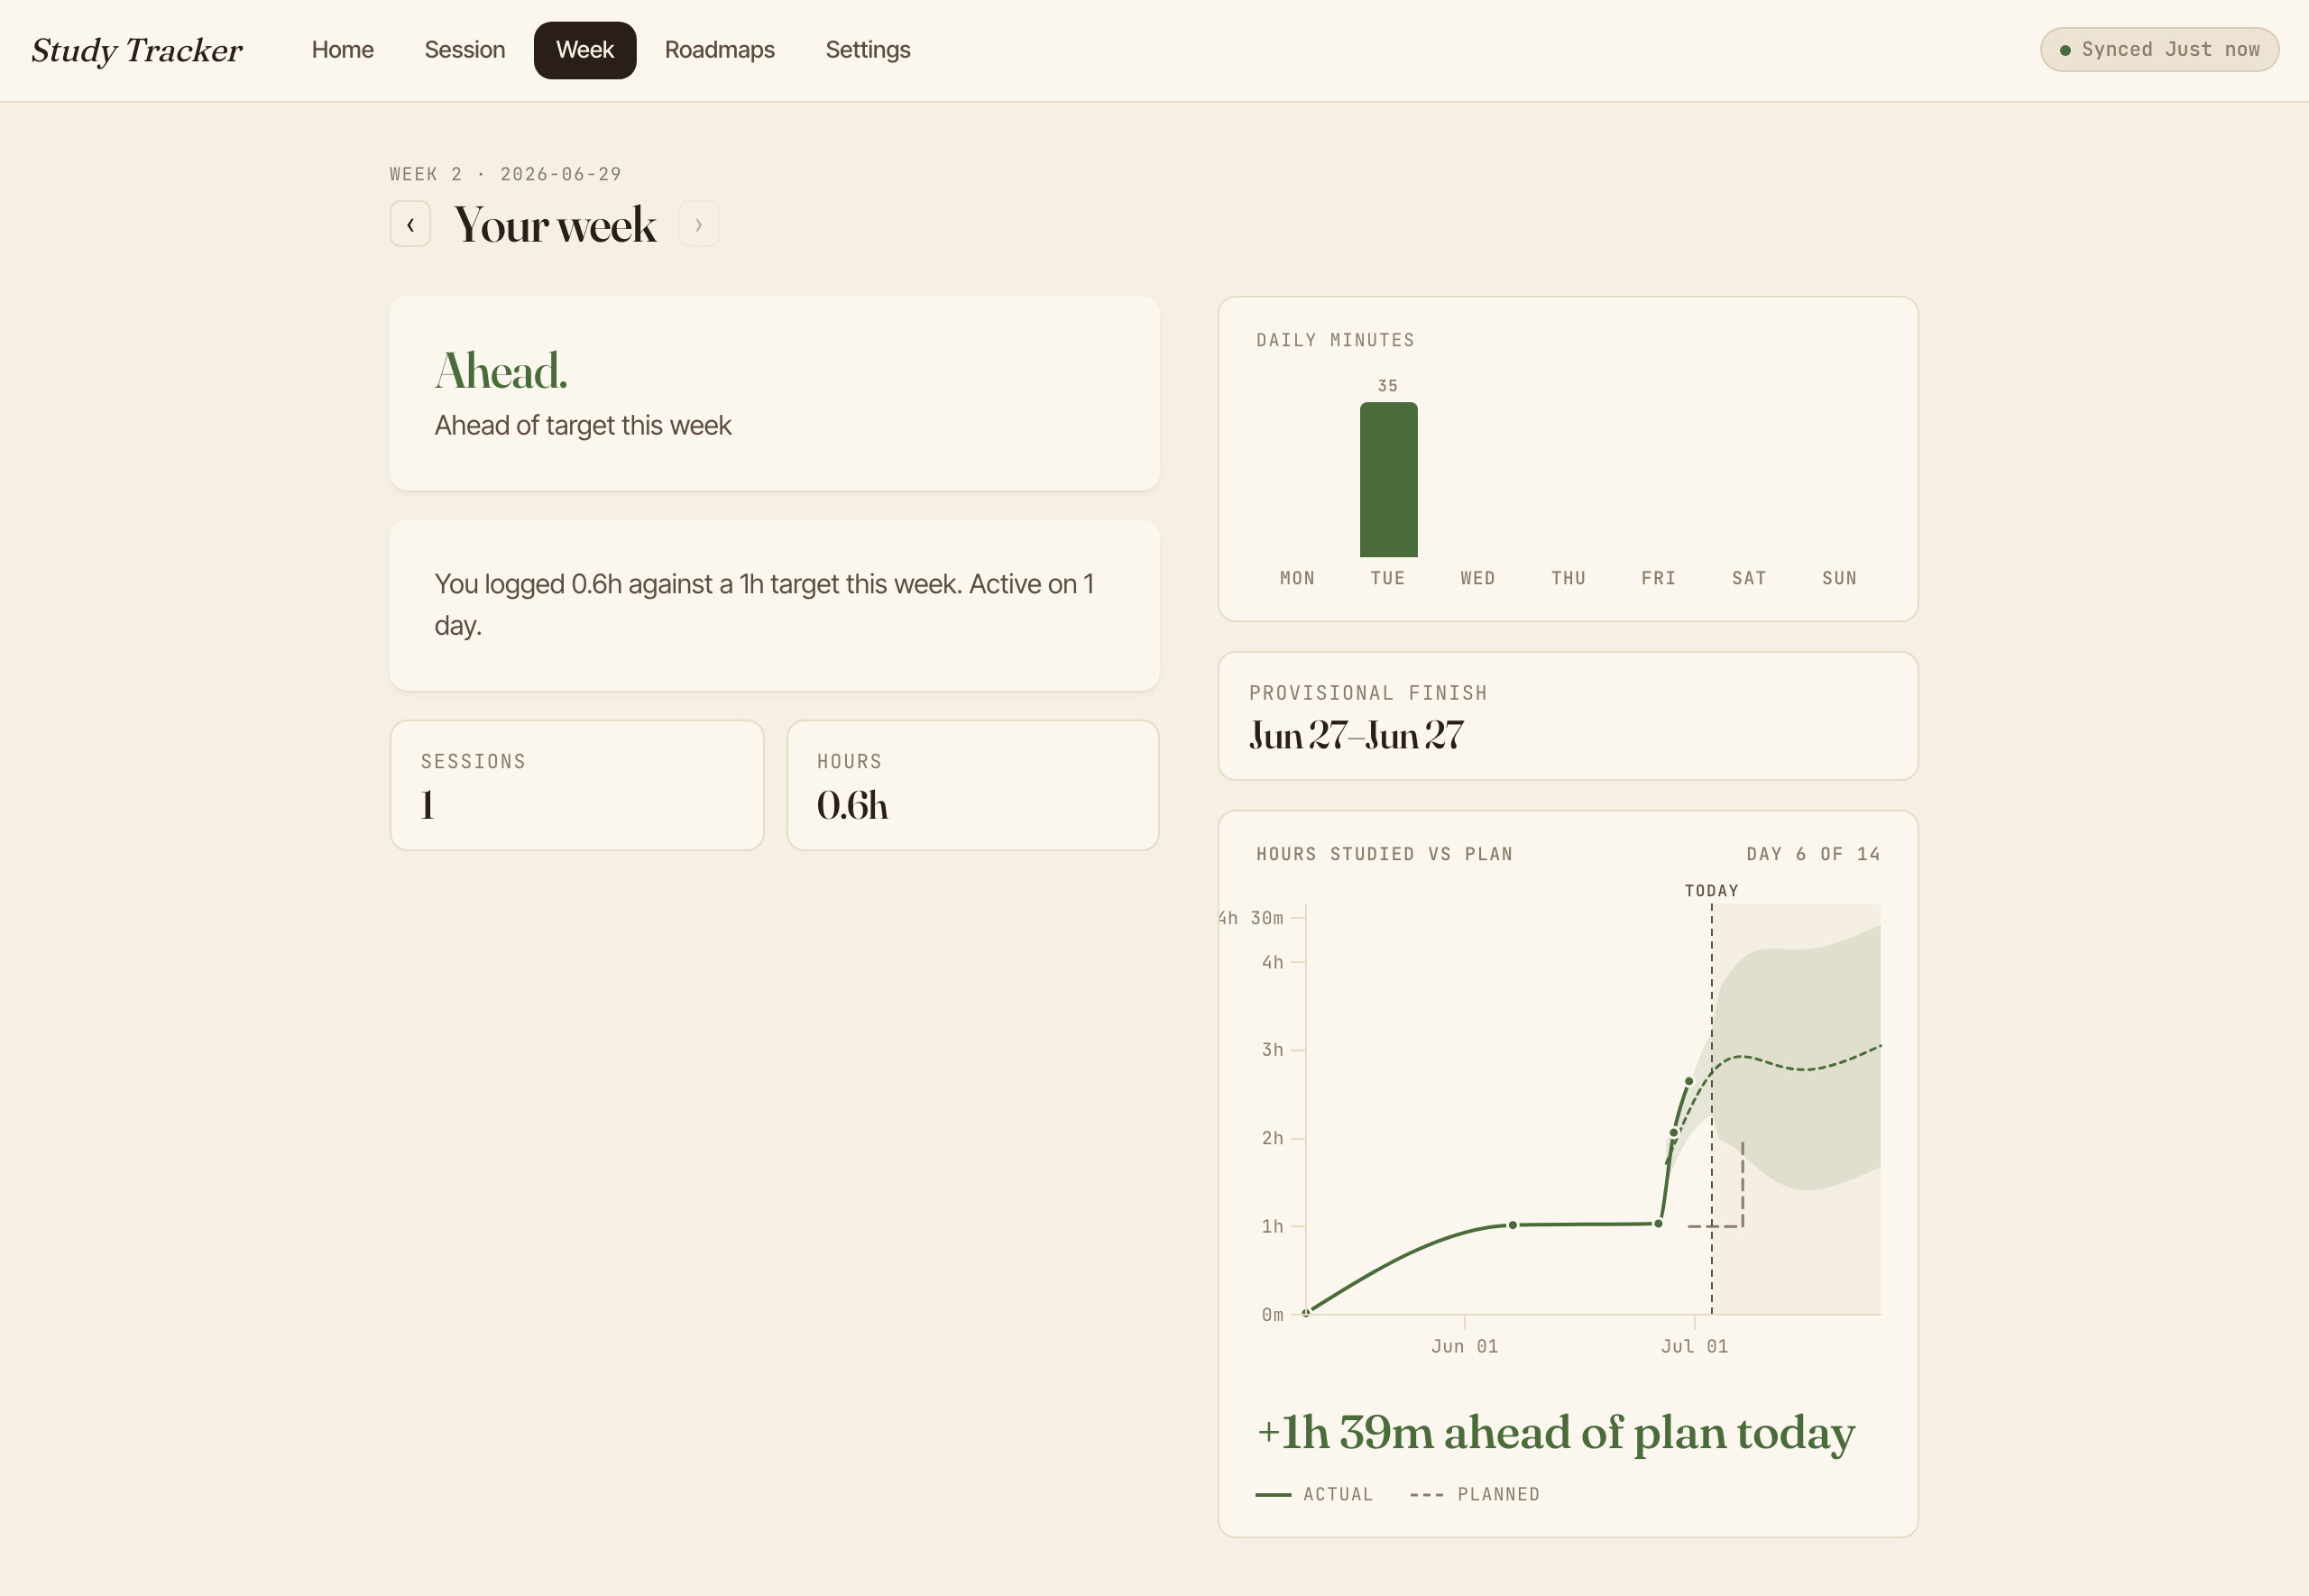
\includegraphics[width=0.85\linewidth, height=0.42\textheight, keepaspectratio]{screenshots/app_week.png}
\caption{The Week view: the week's verdict, the daily-minutes chart, and the burn-up projection.}
\label{fig:app-week}
\end{figure}

\begin{figure}[htbp]
\centering
\includegraphics[width=0.85\linewidth, height=0.42\textheight, keepaspectratio]{screenshots/app_replan.png}
\caption{The Replan screen: three levers to adjust the plan when the projection diverges from the deadline.}
\label{fig:app-replan}
\end{figure}

\begin{figure}[htbp]
\centering
\includegraphics[width=0.85\linewidth, height=0.42\textheight, keepaspectratio]{screenshots/app_roadmap.png}
\caption{The Roadmap calendar: the plan shown as a month grid of bookings.}
\label{fig:app-roadmap}
\end{figure}

\begin{figure}[htbp]
\centering
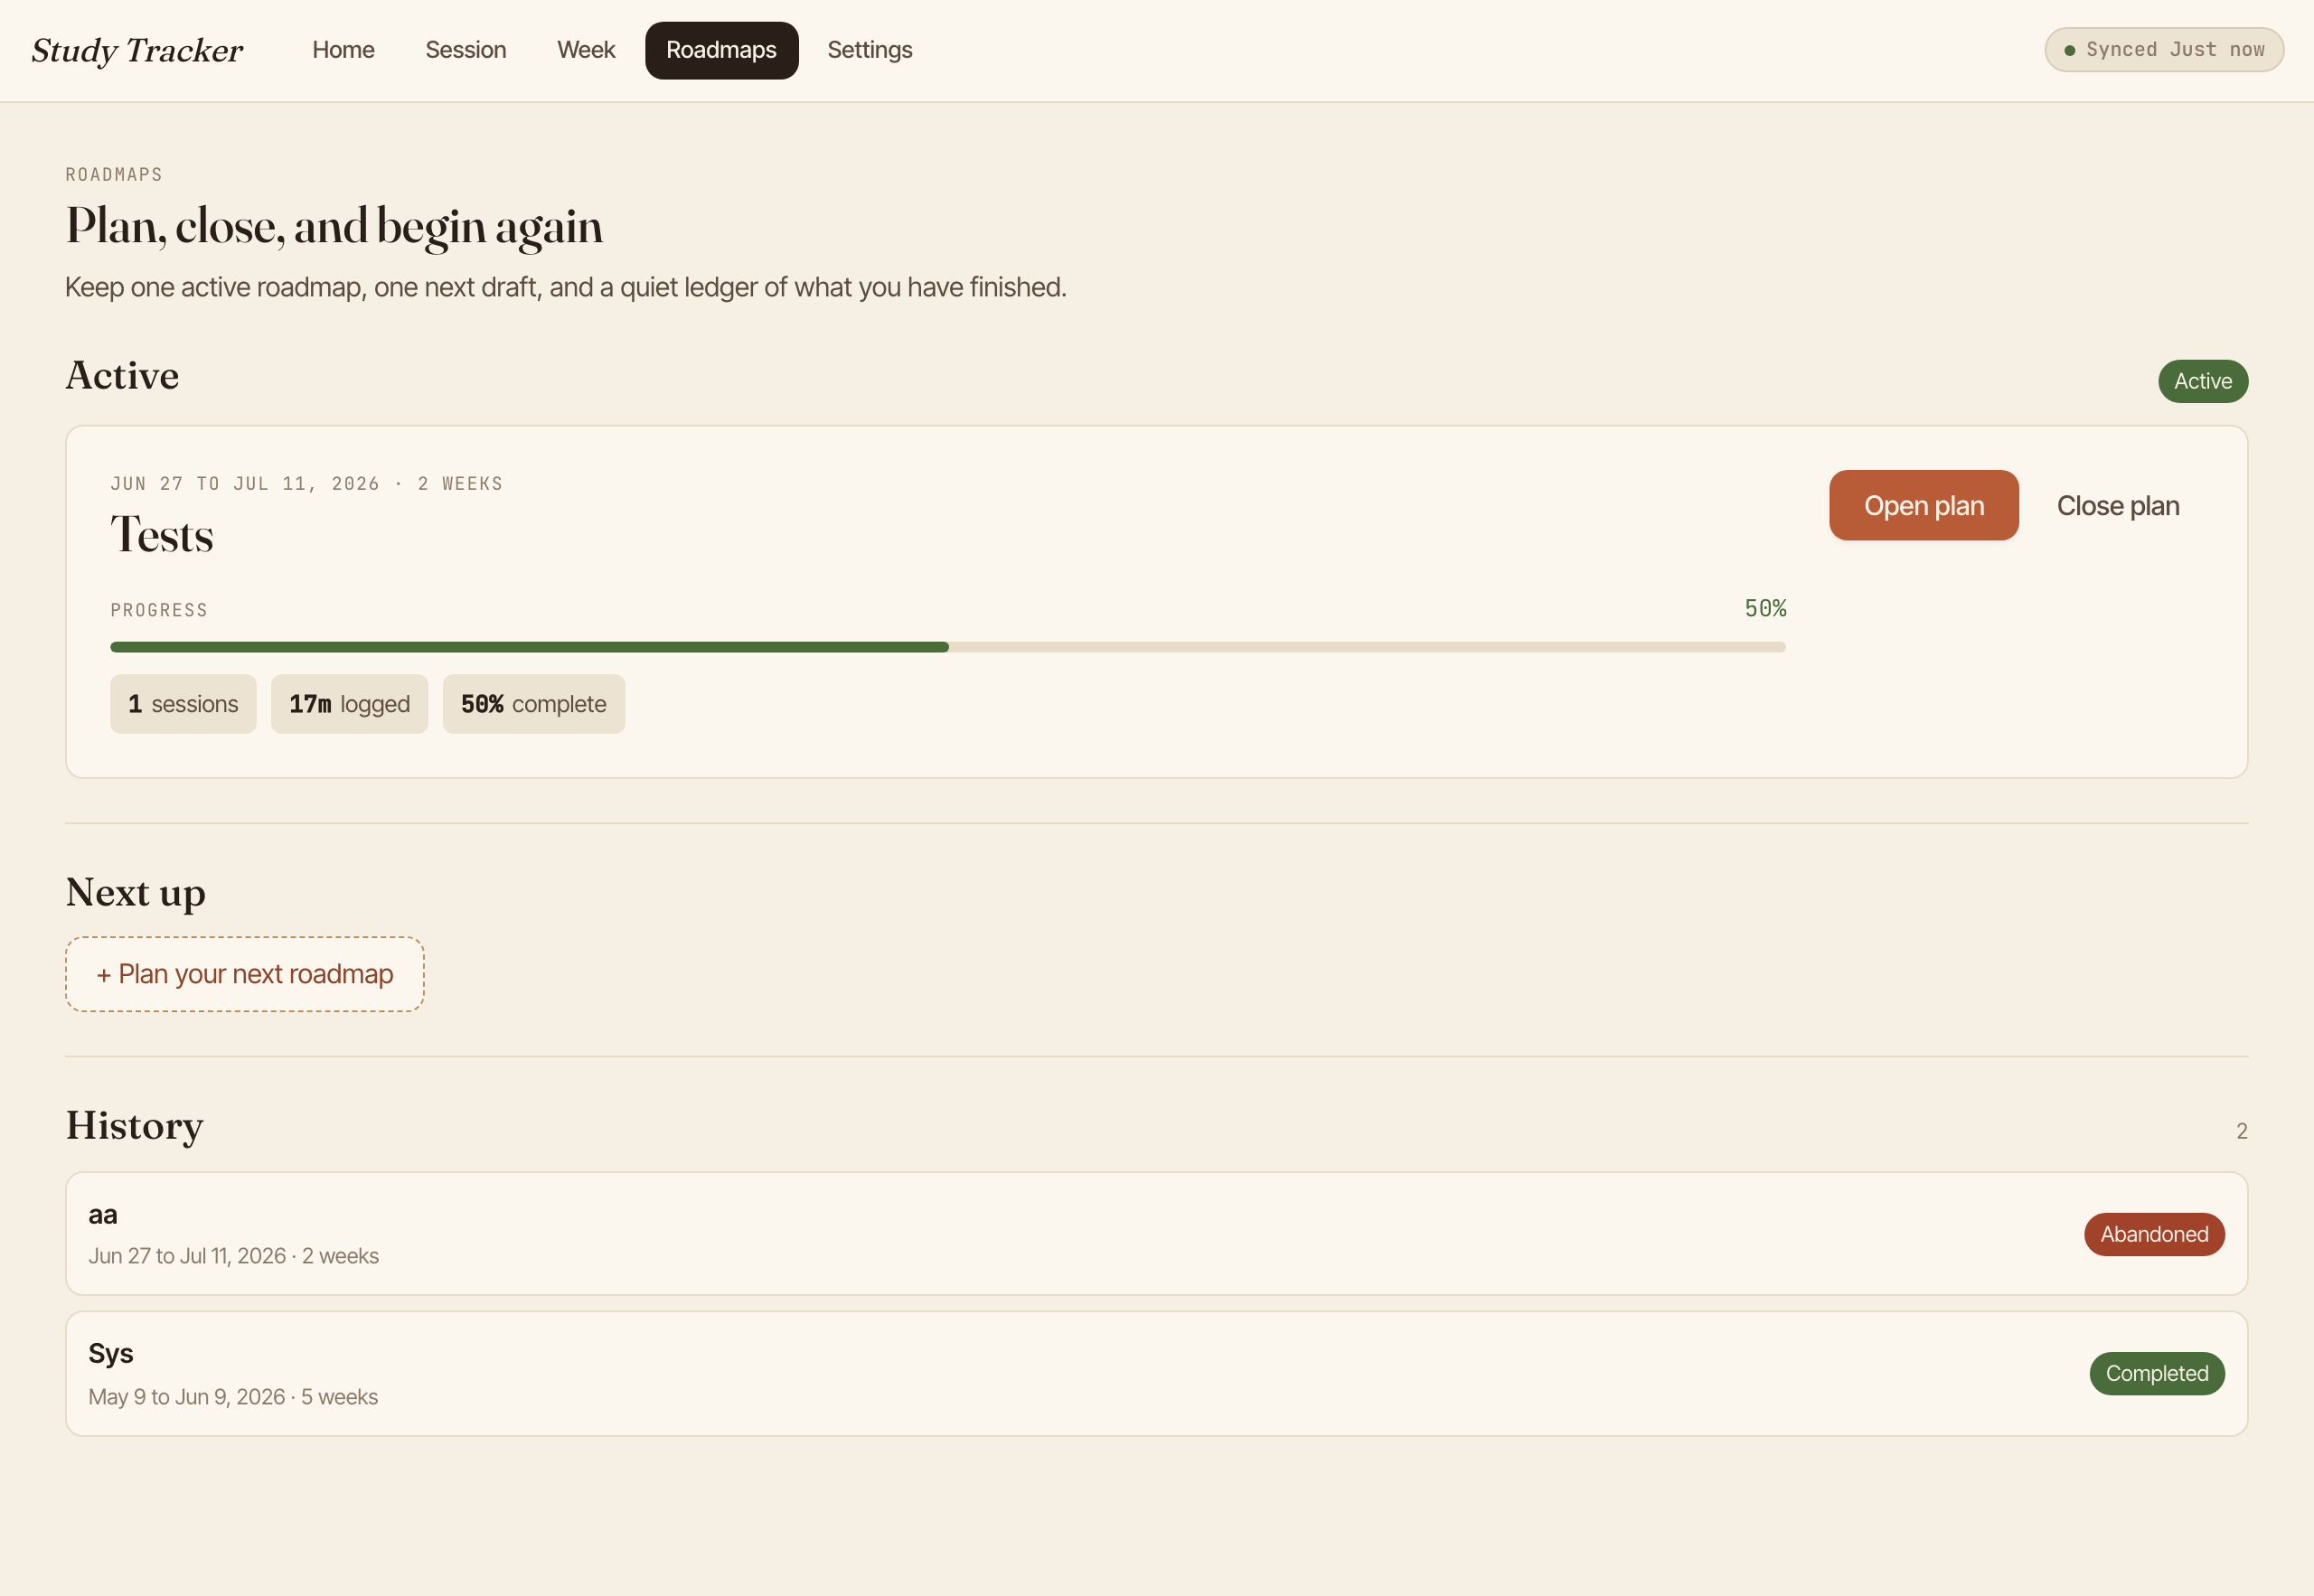
\includegraphics[width=0.85\linewidth, height=0.42\textheight, keepaspectratio]{screenshots/app_roadmaps.png}
\caption{The Roadmaps dashboard: the active plan, drafts, and history over their lifecycle.}
\label{fig:app-roadmaps}
\end{figure}
